\documentclass[sigconf,review,anonymous]{acmart}

\makeatletter
\@ACM@balancefalse
\makeatother
\settopmatter{printacmref=true}
\renewcommand\footnotetextcopyrightpermission[1]{}
\pagestyle{plain}
\raggedbottom

\acmConference[EuroSys '27]{The 22nd European Conference on Computer Systems}{April 19--23, 2027}{Rabat, Morocco}
\acmYear{2027}
\copyrightyear{2027}

\usepackage[T1]{fontenc}
\usepackage{booktabs}
\usepackage{multirow}
\usepackage{siunitx}
\usepackage{graphicx}
\usepackage{amsmath}
\usepackage{xspace}
\usepackage{enumitem}
\usepackage{microtype}
\usepackage{pifont}

\newcommand{\sys}{\textsc{Quiet}\xspace}
\newcommand{\cmark}{\ding{51}}
\newcommand{\xmark}{\ding{55}}
\title{\sys: Dependency-Aware Inference across Isolated Edge-GPU Partitions}

\author{Anonymous Authors}
\affiliation{\institution{Anonymous Institution}\country{Anonymous Country}}
\email{anonymous@example.com}
\keywords{edge AI, dependent inference, MIG, MPS, TensorRT, GPU scheduling}

\begin{CCSXML}
<ccs2012>
  <concept><concept_id>10010520.10010521.10010537</concept_id><concept_desc>Computer systems organization~Distributed architectures</concept_desc></concept>
  <concept><concept_id>10010520.10010520.10010521</concept_id><concept_desc>Computer systems organization~Real-time systems</concept_desc></concept>
  <concept><concept_id>10010147.10010257.10010293</concept_id><concept_desc>Computing methodologies~Machine learning</concept_desc></concept>
</ccs2012>
\end{CCSXML}
\ccsdesc[500]{Computer systems organization~Distributed architectures}
\ccsdesc[500]{Computer systems organization~Real-time systems}
\ccsdesc[500]{Computing methodologies~Machine learning}

\begin{document}
\begin{abstract}
Edge applications increasingly compose opaque neural-network stages, yet GPU
partitioning and serving systems still allocate resources to independent
clients.  This mismatch matters on an integrated edge GPU: an upstream stage
both produces the next stage's input and consumes its end-to-end slack, while
unrelated inference contends for the same physical SoC resources.  Isolated
partitions alone neither carry this dependency nor identify when protected
capacity can be returned.

We present \sys, a dependency-aware runtime for unmodified TensorRT engines on
Jetson AGX Thor.  \sys connects separate MIG CUDA contexts with a
full-coherent registered system-memory activation edge, selects stage
placement and protection under a frozen arrival-to-completion deadline, and
quiesces best-effort work only until the producer publishes its activation.
It then resumes best-effort execution while the consumer runs.  The runtime
modifies neither TensorRT plans, CUDA kernels, nor the GPU driver; every plan,
input, release, activation, output, and measurement trace is hash bound.

Our thermal-normalized ImageNette campaign contains six counterbalanced
sessions and 6,600 requests per system at a frozen $2{,}255.483~\mu$s
deadline.  \sys incurs no misses and a $1{,}902.987~\mu$s p99; its exact
one-sided 95\% deadline-miss bound is 0.0454\%, below the 0.05\% target.
NVIDIA MPS incurs two misses and XSched misses all requests under the same
contract.  Paired across sessions, \sys reduces p99 by $138.508~\mu$s
(95\% CI: $43.798$--$233.217~\mu$s) without a resolved background-goodput
difference.  ImageNette vision and LibriSpeech speech recognition preserve
their reference metrics, and native XSched and Pantheon gates establish two
published-system fidelity paths.  We report a three-load frontier separately
as descriptive evidence because its point-level confidence bounds do not
qualify for the target.  Separately, a nonthermal three-slot Whisper
motivation exposes the dependency-rate crossover: isolated MIG misses 167 of
300 deadlines while \sys misses none; we exclude this cyclic-arrival stress
point from the formal headline.
\end{abstract}

\maketitle
% Generated by analysis/generate_p9_current_figures.py; do not edit by hand.
\newcommand{\PnineApplicationTable}{%
\begin{table}[t]
\centering
\small
\caption{Application-semantic gates. Accuracy is utterance exact-match for ASR; WER is reported separately. Every candidate consumes the recorded inputs and emits a post-completion output trace.}
\label{tab:application-gates}
\resizebox{\columnwidth}{!}{%
\begin{tabular}{lrrrr}
\toprule
Workload & Measured & Reference & QUIET & Delta \\
\midrule
ImageNette ResNet-50 & 90 & 0.8333 acc. & 0.8333 acc. & +0.0000 \\
LibriSpeech Whisper-Tiny & 10 & 0.9000 acc. & 0.9000 acc. & +0.0000 \\
\quad WER & 10 & 0.1127 & 0.1127 & +0.0000 \\
\bottomrule
\end{tabular}%
}
\end{table}
}

\newcommand{\PnineFormalTable}{%
\begin{table}[t]
\centering
\small
\caption{Thermal-normalized ImageNette campaign at the frozen $2{,}255.483~\mu$s production-wall deadline. CP95 is the exact one-sided 95\% upper bound on deadline-miss ratio; the target is 0.05\%.}
\label{tab:formal-campaign}
\resizebox{\columnwidth}{!}{%
\begin{tabular}{lrrrrr}
\toprule
System & Requests & Misses & CP95 DMR & p99 ($\mu$s) & BE rps \\
\midrule
\textbf{QUIET} & 6,600 & 0 & 0.0454\% & 1,902.99 & 249.91 \\
NVIDIA MPS & 6,600 & 2 & 0.0954\% & 2,045.61 & 249.94 \\
XSched (native) & 6,600 & 6,600 & 100.0000\% & 4,351.33 & 97.84 \\
\bottomrule
\end{tabular}%
}
\end{table}
}

\newcommand{\PnineComparatorTable}{%
\begin{table}[t]
\centering
\small
\caption{Native published-system evidence. Pantheon is a separate fidelity gate and is not pooled or ranked with the six-session campaign because its adapter uses a distinct 90-request, integer-$\mu$s deadline contract.}
\label{tab:native-comparators}
\resizebox{\columnwidth}{!}{%
\begin{tabular}{lrrrrl}
\toprule
System & Requests & Accuracy & Misses & p99 ($\mu$s) & Scope \\
\midrule
XSched & 6,600 & 0.8345 & 6,600 & 4,351.33 & formal campaign \\
Pantheon & 90 & 0.8333 & 2 & 4,133 & separate native gate \\
\bottomrule
\end{tabular}%
}
\end{table}
}

\section{Introduction}
\label{sec:introduction}

On-device intelligence is becoming a pipeline rather than a model.  A camera
frame may pass through a backbone and a task-specific head; an audio segment
passes through an encoder before decoding.  These stages exchange activations
that can exceed the original input, and their precedence couples resource
allocation: delay before publication leaves less slack for every downstream
stage.  Meanwhile, consolidating independent analytics is necessary to use an
expensive edge GPU efficiently.

MIG appears to provide the right substrate.  It isolates execution resources
and MIG-local allocations, and Jetson AGX Thor exposes fixed profiles suitable
for placing different stages~\cite{nvidiathormig}.  Its abstraction, however,
ends at each CUDA context.  A device allocation in one instance is not the
input object of another, and the hardware does not express that capacity
protected for a producer may be returned once its output becomes visible.
MPS can regulate active-thread shares inside an instance, but it does not
retract work already submitted by an independent client~\cite{nvidiamps}.
Consequently, isolation and quota control do not by themselves enforce a
pipeline deadline.

Existing serving abstractions inherit the same independent-client boundary.
GSLICE and gpulet tune spatial shares and placement for services
~\cite{gslice2020,gpulet2022}.  Kernel- and stream-level schedulers expose
finer control, but still need a first-class activation edge and an
arrival-to-completion contract to decide \emph{when} that control is safe.
The missing abstraction is therefore not another partition size.  It is the
lifecycle of a dependent request across isolated partitions.

\begin{figure*}[t]
  \centering
  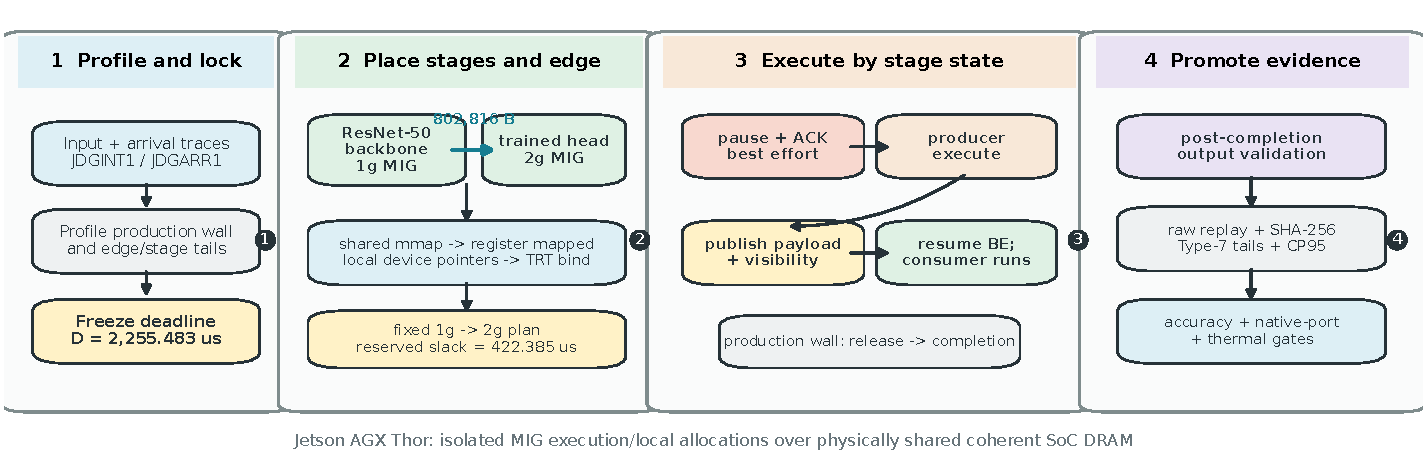
\includegraphics[width=\textwidth]{figures/p9-quiet-overview.pdf}
  \caption{The architecture and procedure of \sys.  The planner freezes a
  workload-specific deadline, places the two validated stages and their
  activation edge, and serializes the resulting contract.  At runtime,
  best-effort work is protected only through producer publication.  Accuracy,
  raw-replay, native-port, and thermal gates determine which results may be
  promoted.  The current production path is a two-stage chain, not a
  general-DAG runtime.}
  \Description{Four numbered modules show profiling and deadline locking,
  stage and activation-edge placement, publication-scoped execution, and
  evidence promotion on Jetson AGX Thor.}
  \label{fig:quiet-overview}
\end{figure*}

Jetson AGX Thor also supplies the key opportunity.  Although its MIG instances
isolate GPU execution and local allocation, the CPU and integrated GPU share
physical SoC DRAM.  A system-memory region can be mapped into separate
processes, registered in each selected CUDA context, and bound directly to
TensorRT I/O.  This preserves isolation while making the \emph{same physical
activation bytes} addressable by both stages.  The opportunity does not make
communication free: visibility, notification, shared-SoC contention, and
consumer queueing remain on the critical path.  A useful runtime must measure
these effects jointly and couple them to admission.

This observation raises our central question:
\begin{quote}
\emph{Can an edge runtime carry a real activation across isolated GPU
partitions, reclaim producer capacity, and still meet a frozen request
deadline?}
\end{quote}

We answer with \sys, whose procedure is shown in
Figure~\ref{fig:quiet-overview}.  \sys first profiles a concrete two-stage
TensorRT chain and freezes a deadline from independent calibration.  It then
selects the MIG UUIDs, quotas, edge transport, protection scope, and admission
state before creating GPU processes.  The data plane starts from a shared
\texttt{mmap}.  Each process invokes \texttt{cudaHostRegisterMapped}, then
obtains a local pointer with \texttt{cudaHostGetDevicePointer}.  TensorRT
binds that pointer directly.  We call this
path the \emph{full-coherent registered system-memory activation edge}.  It is
neither a CUDA managed-memory path nor a shared device allocation.

At runtime, an operational arrival trace releases each request independently
of the previous request's acknowledgement or validation.  \sys drains and
pauses the best-effort tenant, executes the producer, publishes the activation,
and immediately resumes the tenant while the consumer executes.  Checksums
and output capture occur after the production-completion boundary.  Thus, the
reported latency includes queueing and protection but excludes work performed
solely to validate the experiment.

NVIDIA MPS is our vendor baseline.  A native XSched path supplies the
fine-grained baseline~\cite{xsched2025}.  A separately scoped native Pantheon
gate~\cite{pantheon2024} uses a distinct integer-microsecond adapter contract
and is not pooled with the six-session table.  Orion~\cite{orion2024} remains
outside numeric claims because its upstream differential decision gate is
incomplete.  BLESS~\cite{bless2025} and independent-service provisioners
remain structural comparisons when their published mechanisms cannot execute
the identical dependency contract.
DeepPlan~\cite{deepplan2023} motivates direct host access, while edge runtimes
such as Miriam and Pantheon~\cite{miriam2023,pantheon2024} establish
complementary model-aware and preemptive designs.  We retain their names only
for faithful native mechanisms, never for a local approximation.

Our evaluation produces four results.  First, both a 90-request ImageNette
classification gate and a 10-request LibriSpeech ASR gate preserve their
reference metrics; the latter produces byte-identical output traces.  Second,
same-activation causal replay shows that precedence changes shared-resource
overlap, not merely copy time: across three exploratory pairs, \sys's
dependent execution has a $2{,}081.286~\mu$s lower mean p99 than the replayed
independent arm.  Third, in the thermal-normalized campaign, \sys is the only
tested system whose 95\% upper deadline-miss bound qualifies for the 0.05\%
target.  Fourth, offered-load points reveal the expected statistical boundary:
three 3,300-request points can describe behavior but cannot certify a
0.05\% target when zero misses alone would still yield a 0.0907\% upper bound.

\noindent\textbf{Contributions.}
\begin{enumerate}[leftmargin=*,itemsep=1pt,topsep=2pt]
  \item We identify \emph{dependency blindness} as a missing systems
  abstraction between isolated GPU partitions: placement must include the
  activation edge and protection must follow publication state.
  \item We implement a full-coherent registered system-memory activation edge
  for unmodified TensorRT engines in separate Thor MIG contexts, together with
  request-indexed activation replay and post-completion output validation.
  \item We design a hash-bound planner and stage-aware quiescence protocol that
  reserves a measured joint tail and resumes best-effort work immediately
  after producer publication.
  \item We provide two real-application semantic gates, two faithful
  published-system paths, request-level raw replay, exact deadline-miss
  confidence bounds, and six counterbalanced thermal sessions.
\end{enumerate}

The remainder of the paper describes the hardware and scheduling mismatch
(\S\ref{sec:background}), the \sys design (\S\ref{sec:design}) and
implementation (\S\ref{sec:implementation}), and the evidence and its explicit
promotion boundaries (\S\ref{sec:evaluation}).

\section{Background and Motivation}
\label{sec:background}

\subsection{Partitioned Inference on a Coherent Edge SoC}

Thor's MIG profiles divide GPU execution resources and isolate MIG-local
allocations.  We use one 1g instance with eight streaming multiprocessors and
one 2g instance with twelve.  Each stage owns a distinct CUDA context and an
opaque, serialized TensorRT engine.  This is a useful fault and resource
boundary, but it is not an inter-stage data plane: a device allocation made by
the producer cannot simply become the consumer's binding.

The integrated memory architecture creates a second, orthogonal property.
CPU mappings and the iGPU ultimately reach the same physical SoC DRAM.  CUDA
can register a page-aligned system-memory range in each process and return a
context-local device pointer for that range.  The producer and consumer
therefore use different virtual device pointers to the same physical payload.
MIG isolation remains intact because neither process imports the other's
MIG-local allocation.

This distinction determines our terminology.  The implemented transport is a
\emph{full-coherent registered system-memory activation edge}.  It is not
\texttt{cudaMallocManaged}/UVM.  It also does not imply free communication:
the request still incurs publication ordering, a CPU notification, consumer
wakeup, and contention on shared SoC resources.  \sys treats those costs as
measured properties of a placement rather than attributes of the memory API.

\subsection{Why Independent-Client Provisioning Falls Short}

Consider a producer $P$, a consumer $C$, and an unrelated best-effort tenant
$B$.  A fixed spatial policy can isolate $P$ and $C$, and an MPS quota can
limit $B$ within the producer instance.  Neither policy represents the
precedence $P\prec C$.  Three consequences follow.

\textbf{The edge is outside the resource model.}
The provisioner can select two partitions without knowing the payload size,
transport, or notification tail between them.  Treating these quantities as a
constant copy term is incorrect on a coherent SoC: cache state and overlapping
GPU or memory traffic can dominate the measured handoff.

\textbf{Protection has no release event.}
Pausing $B$ for the complete request protects both stages but wastes the
interval in which only $C$ runs on the other partition.  Keeping $B$ active
throughout the request permits already-issued work to delay $P$.  The
activation's publication is the earliest event that is both safe and useful
for returning the producer's capacity.

\textbf{Tail objectives are not end-to-end SLOs.}
Adding independently measured p99s is not a p99 bound: tail events need not
occur on the same request.  Admission must use either the measured joint
arrival-to-completion distribution or an explicit risk allocation, and it
must include gate acquisition and queue delay.

\begin{table}[t]
  \centering
  \small
  \caption{Scheduling scope under the dependent two-stage contract.  A cross
  means that the abstraction does not expose the property as a first-class
  contract; it does not preclude composing additional software around it.}
  \label{tab:abstraction-gap}
  \resizebox{\columnwidth}{!}{%
  \begin{tabular}{lcccc}
    \toprule
    Abstraction & Isolated placement & Explicit activation & Publication release & E2E admission \\
    \midrule
    MIG / MPS & \cmark & \xmark & \xmark & \xmark \\
    Independent-service provisioner & \cmark & \xmark & \xmark & partial \\
    Kernel / stream scheduler & partial & \xmark & \xmark & partial \\
    \textbf{\sys} & \cmark & \cmark & \cmark & \cmark \\
    \bottomrule
  \end{tabular}%
  }
\end{table}

Table~\ref{tab:abstraction-gap} summarizes the gap.  \sys does not replace
hardware isolation or fine-grained scheduling.  It adds the dependency,
publication, and deadline contracts required to use those mechanisms for a
cross-partition pipeline.

\subsection{A Request-Rate Crossover}

Isolation is sufficient when the dependent stages fit comfortably inside one
instance.  Our ImageNette control is in this regime: its consumer is much
shorter than its producer, and colocating both stages on 2g avoids an
unproductive split.  The relevant counterexample is a pipeline with substantial
work on both sides of the edge and more than one request in flight.

We test that counterexample with the real encoder and decoder of
Whisper-Tiny~\cite{radford2022whisper}.  Three activation slots allow encoder
request $i+1$ on 1g to overlap decoder request $i$ on 2g.  Every arm replays the
same labelled LibriSpeech windows, $2{,}304{,}000$-byte FP32 activation,
19-request/s release schedule, $250$-ms deadline, saturated DistilBERT
best-effort tenant, and output oracle.  We rotate the treatment order over
three sessions of 100 measured requests.  NVIDIA MIG places both critical
stages on 2g and isolates best effort on 1g; static NVIDIA MPS splits the
stages but continuously shares 1g; \sys uses the same split and protects 1g
only through producer publication.  TensorRT requires profile-specific
encoder plans, so we rebuild and hash-bind 1g and 2g FP32 plans while holding
the model, decoder plans, inputs, and outputs fixed.

\begin{figure*}[t]
  \centering
  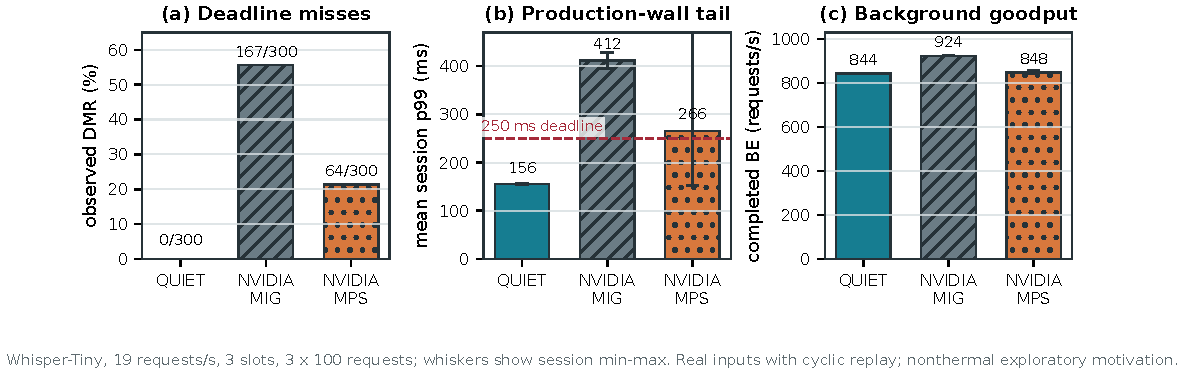
\includegraphics[width=\textwidth]{figures/p9-whisper-asr-mig-crossover.pdf}
  \caption{Nonthermal Whisper-ASR motivation at 19 requests/s.  Every panel
  repeats \sys, NVIDIA MIG, and NVIDIA MPS in the same order.  Bars aggregate
  three 100-request sessions; p99 and best-effort whiskers show the session
  range.  The twelve real windows are cyclically replayed for performance and
  do not constitute additional accuracy coverage.}
  \label{fig:asr-mig-crossover}
  \Description{Three bar charts compare QUIET, NVIDIA MIG, and NVIDIA MPS.
  QUIET has zero of 300 deadline misses and 156 ms mean session p99.  MIG has
  167 misses and 412 ms p99.  MPS has 64 misses and 266 ms p99.  MIG has the
  highest background goodput; QUIET and MPS have similar background goodput.}
\end{figure*}

Figure~\ref{fig:asr-mig-crossover} exposes the crossover.  MIG misses 167 of
300 deadlines because co-located stages sustain only 17.791 requests/s and
queue p99 reaches 241.104 ms.  Static MPS misses 64 requests, all in one
session.  \sys records 0/300 misses, a 155.581-ms mean session p99, and 18.732
critical requests/s.  Its 843.645 best-effort requests/s differs by only
$-0.5\%$ from static MPS, while MIG preserves 924.073 requests/s by dedicating
1g to best effort.  All nine output traces are byte-identical.  The result
therefore identifies a dependency-rate regime in which rigid isolation is not
the correct placement and ungated sharing is not stable enough.

The architecture and dependency are deployment-real, but the load point is
only partially so.  Thor officially supports concurrent hardware-isolated tenants in this 1g+2g
geometry~\cite{nvidiathormig}; Whisper is a real 30-second-window
encoder--decoder application, and prior work adapts it to live streaming
service~\cite{machacek2023whisperstreaming}.  Our fixed 19-request/s trace can
represent a multi-channel edge gateway or queued transcription service, but it
is a cyclic replay rather than a measured deployment arrival trace.  The
250-ms deadline is an internal inference budget, not a universal ASR response
target.  We consequently use Figure~\ref{fig:asr-mig-crossover} as nonthermal
motivation, not as a formal headline or accuracy expansion.

\subsection{Execution and Evidence Contract}

For request $i$, let $a_i$ be its actual release and $c_i$ the consumer's
production completion.  The measured response is
\begin{equation}
  L_i = c_i-a_i ,
  \label{eq:production-wall}
\end{equation}
and a deadline miss occurs when $L_i>D$.  A declared release is never moved
forward to hide a busy pipeline.  If the runtime reaches it late, the
difference is recorded as queue delay and remains inside $L_i$.  Checksum and
output-oracle work occurs after $c_i$; its duration is recorded but cannot
inflate the service metric or extend the protection interval.

The current promoted runtime executes a two-stage chain with at most one
request in flight in each process.  A separate three-slot, external-process
ring validates ownership, wraparound, backpressure, bounded timeout, and stale
slot reclamation, but it is not yet the production TensorRT path.  Likewise,
the planner schema validates larger DAG topologies, while the executed
application remains two-stage.  We therefore make neither a general-DAG nor a
multi-inflight performance claim.

These constraints lead to four design requirements:
\begin{enumerate}[leftmargin=*,itemsep=1pt,topsep=2pt]
  \item \textbf{R1: exact payload semantics.}  Both stages must bind the full
  request-specific activation, with no token or constant-payload substitute.
  \item \textbf{R2: publication-scoped protection.}  The best-effort tenant
  must be acknowledged idle before producer release and resumed immediately
  after payload visibility.
  \item \textbf{R3: joint-tail admission.}  Placement and quotas must fit a
  frozen arrival-to-completion deadline using a promotable tail model.
  \item \textbf{R4: fail-closed evidence.}  A stale engine, binary, input,
  release trace, plan, or output must invalidate the result rather than
  silently changing its contract.
\end{enumerate}

\section{\sys Design}
\label{sec:design}

\subsection{Overall Procedure}

Figure~\ref{fig:quiet-overview} follows the same four steps in deployment and
measurement.  First, \sys profiles a concrete workload and freezes its
deadline independently of the evaluated treatments.  Second, it evaluates
candidate stage placements, quotas, transports, and protection scopes, then
serializes exactly one feasible plan.  Third, the runtime follows the
activation lifecycle to acquire and release protection.  Finally, an evidence
pipeline replays every request and promotes a number only after its application,
runtime, comparator, and thermal gates pass.

This separation is deliberate.  Calibration cannot observe the treatment
comparison, and the executor cannot rewrite the selected plan after creating a
CUDA context.  The evidence pipeline cannot repair a failed request or
reinterpret an exploratory campaign as formal.  Each transition carries the
hash of the artifact that authorized it.

\subsection{Full-Coherent Registered System-Memory Activation Edge}
\label{sec:edge}

The harness creates a page-aligned shared \texttt{mmap}.  After selecting its
assigned MIG device, each process registers the complete range with
\texttt{cudaHostRegisterMapped} and obtains a local device address through
\texttt{cudaHostGetDevicePointer}.  The producer binds that address to its
TensorRT output; the consumer binds its own address for the same physical
range to its TensorRT input.  Both call
\texttt{IExecutionContext::setTensorAddress} and execute with
\texttt{enqueueV3}.  The hot path therefore materializes the activation once
in coherent system memory and performs no explicit D2H/H2D bounce.

Publication has two parts.  TensorRT completion establishes that the producer
has finished writing the payload; a control message transfers the request
sequence and readiness state to the consumer.  The consumer cannot launch
before receiving that message.  Alternative pinned-bounce, pageable-bounce,
managed-memory, and host-materialization paths remain explicit controls.
\sys never assumes that registration wins: it records producer visibility,
notification, consumer read, and complete wall latency for each candidate.

Payload identity is request scoped.  A capture run stores producer activations
in the \texttt{JDGACT1} format with request ID, shape, size, and checksum.  An
independent causal arm maps those pre-captured bytes before release, whereas
the dependent arm consumes the live publication.  Model, input, activation
bytes, placement, quota, release, background load, request ID, and output
oracle remain fixed; only precedence changes.  This removes CPU
initialization and timed-path copies as causal confounders.

The separate multi-slot implementation uses three payload slots with
\texttt{FREE}$\rightarrow$\texttt{PRODUCING}$\rightarrow$\texttt{READY}
$\rightarrow$\texttt{CONSUMING}$\rightarrow$\texttt{FREE} ownership,
monotonic sequence numbers, backpressure counters, deadlines, peer-liveness
checks, and stale-slot reclamation.  We use it to validate the data-plane
state machine and failures, but retain the lower-inflight production path for
the formal application campaign.

\subsection{Communication-Aware Placement and Admission}
\label{sec:planner}

A candidate plan is
\begin{equation}
  P=(U_P,U_C,q_P,q_B,T,\Gamma),
\end{equation}
where $U_P$ and $U_C$ are the producer and consumer MIG UUIDs, $q_P$ and $q_B$
are producer and best-effort quotas, $T$ is the edge transport, and $\Gamma$
is the protection scope.  The profile contains stage and edge diagnostics, but
the promotable response bound is the Type-7 p99 of the \emph{joint}
arrival-to-completion samples:
\begin{equation}
  R(P)=Q_{0.99}\!\left(\{L_i(P)\}\right).
  \label{eq:joint-tail}
\end{equation}
Legacy sums of component p99s may guide characterization but cannot authorize
a formal plan.

Let $G(P)$ be the measured p99 time needed to close and drain best-effort
submission, and let $H$ be pre-release lookahead.  The uncovered guard is
\begin{equation}
  U(P)=\max(0,G(P)-H).
\end{equation}
The plan is feasible only if
\begin{equation}
  S(P)=D-R(P)-U(P)\ge 0,
  \label{eq:slack}
\end{equation}
the held-out execution also satisfies its p99 gate, and all artifact and
application bindings match.

The current deadline is frozen from two independent 1,100-request calibration
blocks: the pooled p99 is $2{,}050.439~\mu$s and the predeclared 1.10 factor
gives $D=2{,}255.483~\mu$s.  The selected forward placement runs the
ResNet-50 backbone on 1g and its head on 2g.  Its held-out joint p99 is
$1{,}833.098~\mu$s; $G=2{,}000.588~\mu$s and $H=2{,}300~\mu$s make
$U=0$, leaving $422.385~\mu$s of reserved slack.  The serialized plan binds
these values to the exact deadline lock, engines, UUIDs, quotas, payload size,
transport, and producer-only scope.

Planning precedes process creation.  A CLI override that changes a UUID,
transport, quota, protection scope, deadline, or workload hash fails before a
GPU process is started.  This matters because accepting a mismatched plan and
merely annotating the trace would turn admission into an after-the-fact label.

\subsection{Stage-Aware Quiescence}
\label{sec:quiescence}

\begin{figure}[t]
  \centering
  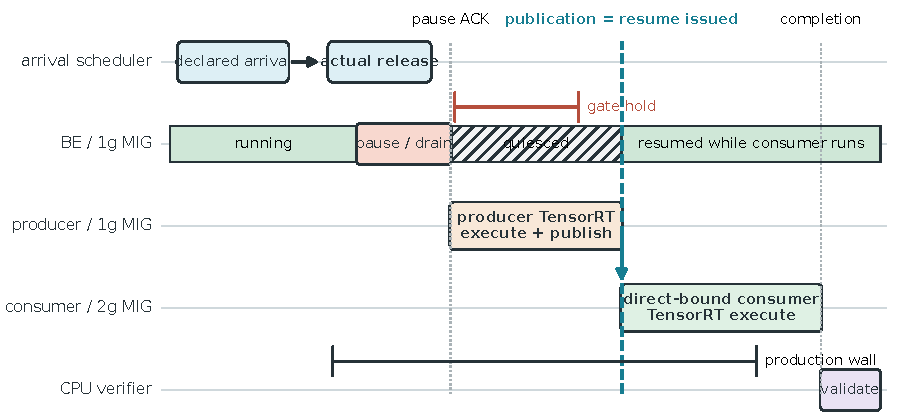
\includegraphics[width=\columnwidth]{figures/p9-stage-timeline.pdf}
  \caption{\sys's request lifecycle.  The operational release precedes gate
  acquisition, so queue and drain delay remain inside the production wall.
  Producer publication is the protection boundary: resume is issued before
  checksum and output validation, and best-effort work overlaps the consumer.}
  \Description{A five-lane timeline shows request release, best-effort drain
  and pause, producer execution and publication, immediate best-effort resume,
  consumer execution, completion, and post-completion validation.}
  \label{fig:stage-timeline}
\end{figure}

Figure~\ref{fig:stage-timeline} shows the runtime protocol.  Before producer
launch, \sys closes future best-effort submission and waits for cooperative
pause acknowledgement.  This is a drain boundary, not a claim of
mid-kernel preemption.  Once acknowledged, the producer executes without new
best-effort work entering its 1g instance.

Producer completion publishes the activation and releases the dependent
consumer.  In the same control transition, \sys issues resume to the
best-effort tenant and records both issue and observation timestamps.  The
consumer then reads the direct-bound payload and executes on 2g while
best-effort work again occupies 1g.  Full-request gating would retain
protection through this interval and forfeit safe work; no gating would expose
the producer tail.  Publication-scoped gating protects exactly the interval
whose interference can delay every downstream stage.

Each event trace records declared arrival, actual release, queue delay,
producer start, publication, consumer start, completion, pause begin and
completion, resume issue and observation, and gate-hold duration.  The
operational \texttt{JDGARR1} scheduler consumes predeclared offsets.  A late
release contributes queue delay rather than shifting the schedule, and neither
an acknowledgement nor post-completion validation determines the next
arrival.

\subsection{Correctness and Evidence Promotion}
\label{sec:evidence}

\sys separates production completion from proof collection without weakening
correctness.  After publication, the producer checks the complete activation
against its request record.  After consumer completion, the harness captures
the complete output and evaluates the application oracle.  A run fails on a
request-sequence mismatch, activation mismatch, output mismatch, stale hash,
missing sensor, or fewer requests than declared.

Promotion has three levels.  A \emph{mechanism control} validates behavior
such as ring recovery or transport direction.  An \emph{exploratory result}
adds repeated measurements but lacks at least one formal condition, such as
thermal normalization or sufficient confidence.  A \emph{formal result} binds
the current binary and engines, operational releases, application inputs and
outputs, balanced treatment order, independent sessions, thermal sensors, and
an exact deadline-miss confidence bound.  Results never cross levels during
aggregation.

\section{Implementation}
\label{sec:implementation}

\subsection{Runtime and Data Plane}

Our prototype runs on Jetson Linux R39.2 with CUDA 13.2 and TensorRT 10.16.2.
Bootstrap code creates Thor profile 78 (1g) and profile 83 (2g), validates the
resulting devices, and starts a private MPS server for best-effort work on the
1g instance.  CPU affinity places the control path, critical workers, and load
generator on disjoint cores.

The C++ runtime forks separate producer and consumer processes around a shared
page-aligned mapping.  Each child selects its assigned MIG UUID before
registering the mapping.  Registration uses a move-disabled RAII wrapper.
Both normal and exceptional teardown call
\texttt{cudaHostUnregister}.
Tensor sizes are derived from engine metadata with overflow and dynamic-shape
checks; every CUDA and TensorRT error propagates to the parent rather than
being converted to a successful trace.

The formal vision workload binds a $[1,1024,14,14]$ FP32 backbone output, an
802,816-byte payload, directly to the trained classification head.  A learned
ResNet10 detector split uses a 1,884,160-byte activation, and Whisper-Tiny uses
a 2,304,000-byte encoder activation.  These paths carry complete tensors.
Shape-compatible synthetic projections exist only as transport controls and
are never presented as application-accuracy results.

The standalone ring uses three slots in a shared descriptor and payload
mapping.  Atomic sequence and ownership fields prevent ABA reuse; producers
observe backpressure rather than overwrite \texttt{READY} data.  Timeout and
peer-death paths inspect process liveness, reclaim stale ownership, and unpause
surviving tenants.  Normal wraparound and delayed-consumer tests complete
without mismatches; the timeout test exits within its bound, and injected
consumer death records a stale reclaim.  Integrating this ring with the
formal vision TensorRT path is future work.  The Whisper motivation path uses
a narrower three-slot credit window: each transfer carries a dense slot index,
the consumer acknowledges only after decoding, and the producer must receive a
credit before reusing that slot.  TensorRT rebinds the encoder output and
decoder input to the selected registered range.  This path provides real-model
request overlap and backpressure, but it does not claim the standalone ring's
timeout and stale-owner recovery contract.

\subsection{Release, Protection, and Trace Collection}

The \texttt{JDGARR1} reader validates each request ID and input digest before
execution.  The release loop waits on the recorded monotonic offset, preserves
the declared timestamp, and records the actual timestamp and queue delay.
Pause and resume use cooperative process control.  The runtime records
\texttt{pause\_begin}, \texttt{pause\_complete},
\texttt{publication}, \texttt{resume\_issued}, and
\texttt{resume\_observed} for every request.
The exploratory Whisper runner uses verified \texttt{SIGSTOP} and
\texttt{SIGCONT} control around the same producer's publication boundary and
records gate hold and acquisition separately; this distinction is retained in
its provenance.

The publication code sends the dependent consumer's transfer record and then
resumes producer-scoped best-effort workers.  Producer checksum calculation
follows this transition.  Consumer completion closes the production wall;
output capture and oracle comparison follow completion.  CSV rows retain
producer compute and copy time, notification, consumer copy and compute time,
validation time, wall latency, deadline classification, and lifecycle
timestamps, so an analyzer can recompute both the metric and its boundary.

Activation capture writes a binary trace.  Its \texttt{JDGACT1} records carry
the request index, payload bytes, and digest.  Independent-mode startup
requires this file and rejects a missing, malformed, or shape-incompatible
trace.  The consumer binds the selected replay record before release and
validates the live producer activation against the same record after
publication.  This ensures that the independent arm changes precedence alone.

\subsection{Planner and Reproducibility}

Python tools freeze calibration, build candidate plans, execute
counterbalanced sessions, monitor \texttt{tegrastats}, and replay raw evidence.
The lock records the runtime binary, source, TensorRT engines, producer input,
and operational release hashes.  The selected plan adds UUIDs, quotas,
transport, protection scope, joint-tail method, guard, lookahead, and residual
slack.  A prelaunch verifier rejects any mismatch.

Aggregation recomputes Type-7 percentiles from request-level CSV files and the
exact one-sided Clopper--Pearson upper deadline-miss bound.  It validates
per-session request counts, deadline decisions, input and output containers,
treatment order, required \texttt{soc012} and \texttt{tj} temperatures, and
the VDD\_GPU rail.  The paper-figure generator repeats the artifact SHA-256
checks and raw p99 replay before emitting a PDF or table.

\subsection{Published-System Ports}

We distinguish an executable native path from a local behavioral
approximation.  A published name is admitted only when the pinned artifact's
scheduler and runtime execute the measured request.  The XSched port retains
its CUDA shim, scheduling-unit queues,
and policy at upstream commit \texttt{bd494cb7a729}; its Thor patch adds CUDA 13
and \texttt{cuLaunchKernelEx} compatibility without replacing the scheduler.
The Pantheon gate retains the online runtime, two-tier stream priorities,
model repository, and chunked modules at upstream commit
\texttt{1caa4321fe9f}.

Orion's local port executes its operation queues and resource profiles, but
its upstream differential-decision evidence remains incomplete.  We report
its measured application and historical results with that scope attached
rather than pooling them with the formal campaign.  BOER, ParvaGPU, GSLICE,
gpulet, and BLESS likewise retain their executed positive controls, diagnostic
numbers, or compatibility failures.  Only rows whose original runtime also
executes the same model, input, release, output, and deadline contract enter a
direct rank.  This rule prevents fixed quotas or request-level gating from
being relabeled as a published system without hiding experiments that ran.

\section{Evaluation}
\label{sec:evaluation}

We evaluate five questions:
\begin{enumerate}[leftmargin=*,itemsep=0pt,topsep=2pt,label=\textbf{Q\arabic*:}]
  \item Does the cross-partition pipeline preserve application semantics?
  \item Why must dependency and transport be measured as a scheduling
  contract rather than a copy constant?
  \item Does \sys meet a frozen deadline in the formal campaign, and how does
  it compare with executable baselines?
  \item Are the tail and thermal results stable across independent sessions?
  \item How do confidence-bounded deadline misses and background goodput
  change with offered load?
\end{enumerate}

\subsection{Experimental Setup}

\textbf{Evidence status.}
A thermal-normalized formal campaign is now bound to the frozen workload,
runtime, arrival trace, and promotion rules described below.

\textbf{Platform.}
All promoted measurements run on one Jetson AGX Thor using a fixed 1g+2g MIG
layout.  The 1g producer exposes eight SMs and shares a private MPS server with
the best-effort tenant; the 2g consumer exposes twelve SMs.  The software stack
is Jetson Linux R39.2, CUDA 13.2, and TensorRT 10.16.2.  Frequencies, process
placement, MIG UUIDs, quotas, and required thermal sensors are frozen by the
campaign manifest.

\textbf{Primary workload.}
The formal workload is a real ResNet-50 ImageNette classifier.  The backbone
runs on 1g and emits the $[1,1024,14,14]$ FP32 tensor described in
\S\ref{sec:implementation}; its trained head runs on 2g.  DistilBERT-SST2
generates best-effort load on 1g at a predeclared open-loop period.  Each
treatment consumes the same request-input trace, \texttt{JDGARR1} operational
release trace, engines, class map, and output oracle.

\textbf{Additional applications and controls.}
We use a real Whisper-Tiny encoder/decoder path on LibriSpeech dev-clean to
test ASR semantics.  A learned ResNet10 backbone/head split supplies the
same-activation causal and transport controls.  The latter is deliberately
not folded into the ImageNette SLO campaign because it has a different model,
payload, and evidence scope.

\textbf{Deadline and sessions.}
Two 1,100-request calibration blocks produce a pooled
$2{,}050.439~\mu$s p99.  Applying the predeclared 1.10 factor freezes
$D=2{,}255.483~\mu$s before treatment execution.  The formal campaign has six
counterbalanced sessions, 1,100 measured requests per system per session, and
6,600 requests per system.  Each session executes NVIDIA MPS, native XSched,
and \sys in one of the frozen balanced orders.  We use request-level samples
for pooled distributions and the six sessions as the statistical units for
paired treatment effects.

\textbf{Metrics and qualification.}
Production-wall latency is Equation~\ref{eq:production-wall}.  We report p50,
p99, p99.9, deadline misses, and completed best-effort requests/s.  Deadline
qualification uses the exact one-sided 95\% Clopper--Pearson upper bound
(CP95) on deadline-miss ratio (DMR), with target $\epsilon=0.0005$.
Zero observed misses are not alone sufficient: the sample count must make
CP95 no greater than $\epsilon$.  All percentiles are Type~7 and replayed from
request-level CSV files.

\subsection{Q1: Application Semantics}

\PnineApplicationTable

Table~\ref{tab:application-gates} reports the two application gates.
ImageNette uses 100 labelled inputs, with ten warmup and 90 measured requests.
The unsplit reference and cross-partition candidate both reach 0.8333
classification accuracy, above the frozen 0.80 threshold, with zero accuracy
delta.  The gate binds each image digest to the external label and records
independent reference and candidate output containers.

Whisper uses twelve LibriSpeech dev-clean utterances, with two warmup and ten
measured requests.  Reference and candidate both reach 0.9000 utterance
exact-match accuracy and 0.1127 WER, below the frozen 0.20 maximum.  Their
complete output containers have the same SHA-256 digest, not merely the same
aggregate score.  Thus, the 2.304-MB activation edge preserves the decoder's
observable transcript for every recorded input.

The thermal campaign repeats a fixed ImageNette trace at greater scale.  All
three systems attain 0.8345 accuracy with zero candidate/reference delta in
every session.  Consequently, the SLO differences below cannot be attributed
to dropping requests from the accuracy calculation or weakening the oracle.

\subsection{Q2: Dependency Changes Contention, Not Only Copy Time}

\begin{figure*}[t]
  \centering
  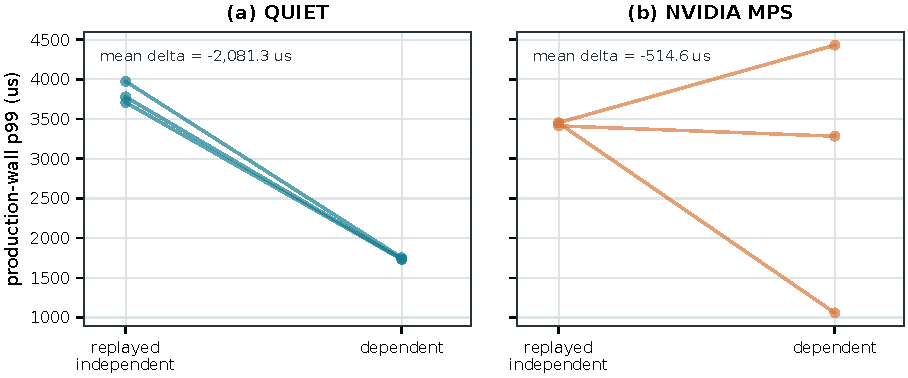
\includegraphics[width=\textwidth]{figures/p9-causal-pairs.pdf}
  \caption{Exploratory same-activation causal replay on the learned ResNet10
  split.  Each line is one sequential pair with 20 measured requests per arm;
  dependent minus independent is the signed effect.  \sys has mean
  $-2{,}081.286~\mu$s (95\% paired-session interval
  $[-2{,}394.953,-1{,}767.619]~\mu$s).  NVIDIA MPS has mean
  $-514.579~\mu$s and an interval spanning zero.  The experiment is not
  thermal normalized and supports a mechanism claim only.}
  \Description{Two paired-line plots compare replayed-independent and
  dependent p99 latency over three repeats for QUIET and NVIDIA MPS.}
  \label{fig:causal}
\end{figure*}

The replayed independent arm binds the request's pre-captured producer
activation before release and permits producer and consumer execution to
overlap.  The dependent arm releases the consumer only after live publication.
All other inputs remain equal.  If the edge were merely an additive copy
penalty, the dependent arm should differ by a stable positive offset.

Figure~\ref{fig:causal} shows the opposite for \sys: serializing on publication
reduces p99 by $1{,}977.575$--$2{,}221.892~\mu$s across all three pairs.
Concurrent independent execution increases shared-SoC contention enough to
outweigh the waiting it removes.  MPS is unstable across pairs: its signed
effects are $+977.388$, $-2{,}391.266$, and
$-129.859~\mu$s, yielding a wide interval that includes zero.  The result
does not claim that dependencies intrinsically improve latency.  It shows
that precedence selects a contention schedule and must therefore be explicit
in the runtime.

A separate 20-request transport control reinforces this point.  For the
1,884,160-byte learned detector edge, registered direct binding has
$2{,}195.508~\mu$s edge p99 and $2{,}908.268~\mu$s wall p99.  Pinned bounce
has a lower $1{,}863.770~\mu$s edge p99 and
$2{,}538.617~\mu$s wall p99, while pageable bounce reaches
$2{,}283.200~\mu$s and $2{,}975.838~\mu$s, respectively.  All three emit the
same output trace.  Notification dominates the registered case in this short
run, whereas copies dominate the pageable case.  Because the experiment is
small and nonthermal, we use it to reject a universal
\emph{registered-is-fastest} assumption, not to rank transports.  \sys instead
profiles the joint tail selected by Equation~\ref{eq:joint-tail}.

\subsection{Q3: Thermal-Normalized Deadline Performance}

\PnineFormalTable

\begin{figure*}[t]
  \centering
  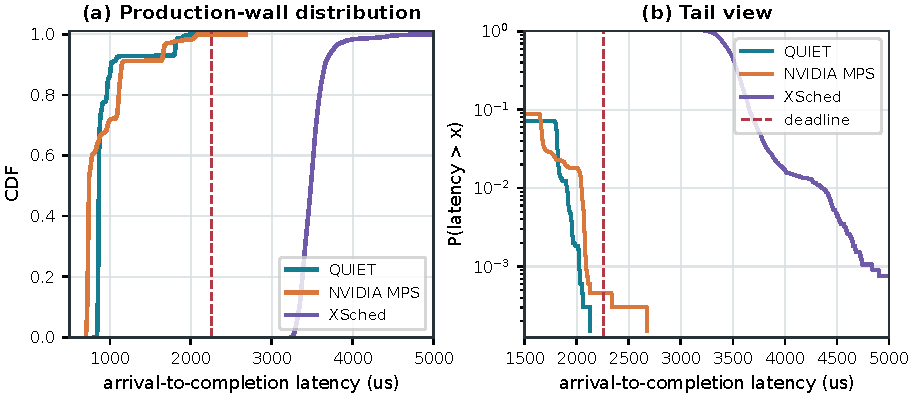
\includegraphics[width=\textwidth]{figures/p9-latency-cdf.pdf}
  \caption{Request-level latency in the six-session thermal-normalized
  ImageNette campaign (6,600 requests/system).  The left panel shows the full
  CDF; the right isolates the tail on a logarithmic survival axis.  The dashed
  line is the frozen $2{,}255.483~\mu$s production-wall deadline.}
  \Description{Two plots compare QUIET, NVIDIA MPS, and XSched latency.  QUIET
  and MPS lie mostly left of the deadline; the XSched distribution lies to its
  right.  The logarithmic tail reveals two MPS misses and no QUIET miss.}
  \label{fig:latency-cdf}
\end{figure*}

Table~\ref{tab:formal-campaign} and Figure~\ref{fig:latency-cdf} give the
formal result.  \sys completes all 6,600 requests before the deadline.  Its
p50, p99, and p99.9 are $863.886$, $1{,}902.987$, and
$2{,}025.643~\mu$s.  The zero-miss CP95 bound is 0.0454\%, which qualifies
for the 0.05\% target.

NVIDIA MPS has a lower $739.887~\mu$s median but a
$2{,}045.606~\mu$s p99 and incurs two deadline misses.  Its observed DMR is
0.0303\%, yet CP95 is 0.0954\%; it therefore does not qualify.  This gap
between median and tail is precisely the behavior that a fixed spatial share
does not expose to a dependent request.  \sys narrows the protected interval
without surrendering the producer tail.

The native XSched port misses all 6,600 requests.  Its median is
$3{,}484.202~\mu$s, and its p99 is $4{,}351.332~\mu$s.  Output accuracy remains
0.8345 with zero delta, so the row is a valid execution of the application but
is infeasible at this lock.  We report the failure rather than retune the
deadline or relabel a local approximation as XSched.

Background throughput separates tail protection from capacity destruction.
\sys completes 249.909 best-effort requests/s, NVIDIA MPS completes 249.941,
and XSched completes 97.845.  Across the six paired sessions, the \sys-minus-MPS
p99 effect is $-138.508~\mu$s with 95\% interval
$[-233.217,-43.798]~\mu$s.  The paired goodput effect is
$-0.0317$ requests/s with interval $[-0.0988,0.0354]$, which does not resolve
a directional difference.  Thus, the supported claim is a tail reduction at
statistically indistinguishable background goodput, not a throughput gain.

\subsection{Q4: Session and Thermal Stability}

\begin{figure*}[t]
  \centering
  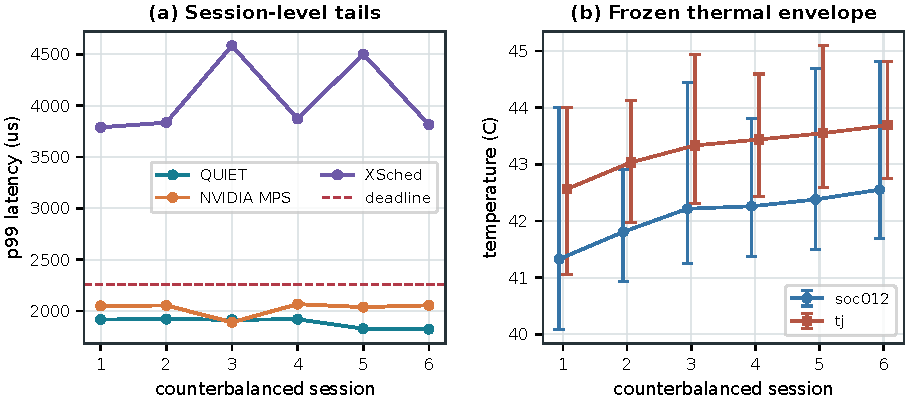
\includegraphics[width=\textwidth]{figures/p9-session-stability.pdf}
  \caption{Independent-session stability.  Panel (a) reports each session's
  p99 against the fixed deadline.  Panel (b) reports mean \texttt{soc012} and
  \texttt{tj} temperatures with observed minimum--maximum bars.  Thermal
  conditions define admissibility; they are not used to rescale latency.}
  \Description{The left plot shows six session p99 values for QUIET, MPS, and
  XSched against the deadline.  The right shows soc012 and tj means with
  observed temperature ranges for the same sessions.}
  \label{fig:stability}
\end{figure*}

Figure~\ref{fig:stability}(a) shows that all six \sys session p99s remain below
$1{,}921~\mu$s.  MPS is also below the deadline at session-p99 granularity,
but its two request-level misses prevent confidence qualification.  XSched is
above the deadline in every session.  The counterbalanced order prevents one
treatment from consistently receiving the first or last thermal position.

Each session contains 430--434 \texttt{tegrastats} samples.  The largest
within-session \texttt{soc012} range is $3.907^\circ$C and the largest
\texttt{tj} range is $2.938^\circ$C, both below the frozen
$8^\circ$C limit.  Cross-session mean temperature changes by at most
$0.910^\circ$C, below the $4^\circ$C envelope, and every sample set contains
the required VDD\_GPU rail.  Figure~\ref{fig:stability}(b) also makes the
slow drift visible rather than hiding it behind an aggregate mean.  The gate
accepts this envelope but does not claim identical temperature.

\subsection{Q5: DMR--Goodput Frontier}

\begin{figure*}[t]
  \centering
  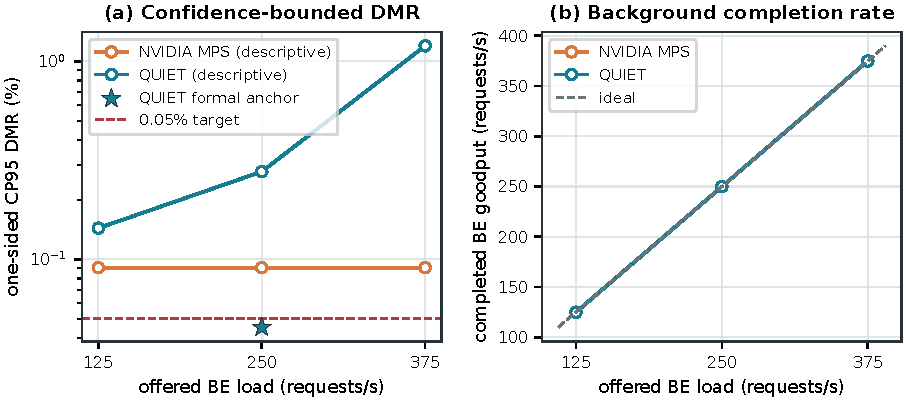
\includegraphics[width=\textwidth]{figures/p9-load-frontier.pdf}
  \caption{Same-workload offered-load sweep.  Hollow markers are descriptive
  three-session points (3,300 requests/point) and are not thermal normalized.
  The star is the separate six-session, thermal-qualified \sys anchor at
  250 requests/s.  No hollow point is used for ranking.}
  \Description{The left log-scale plot shows CP95 deadline-miss bounds versus
  offered load and a qualified QUIET star below the target.  The right plot
  shows QUIET and MPS goodput closely following the ideal line.}
  \label{fig:load-frontier}
\end{figure*}

Figure~\ref{fig:load-frontier} varies best-effort load.  At 125, 250, and
375 offered requests/s, \sys completes 124.941, 249.908, and 374.897 rps.
MPS completes 124.950, 249.888, and 374.868 rps.  Both track the ideal line,
so goodput alone makes them appear indistinguishable.

Confidence-bounded DMR exposes a different picture.  MPS observes no misses at
all three points, but 3,300 requests only bound DMR by 0.0907\%, above the
0.05\% target.  \sys observes 1, 4, and 29 misses, producing CP95 bounds of
0.1437\%, 0.2772\%, and 1.1963\%.  The 375-request/s point also exceeds the
selected plan's gate bound.  These points describe overload behavior; the
campaign's \sys star is the only statistically qualified point because it has
6,600 thermally admitted requests and zero misses.  We do not combine the
three-session 250-request/s point with that anchor because their session and
thermal contracts differ.

\subsection{Executed Comparator Coverage}

\PnineComparatorTable

Table~\ref{tab:native-comparators} includes every comparison implementation
that executed locally.  Evidence class A is the directly ranked formal
campaign: XSched's native path participates in that campaign and is infeasible
at the frozen deadline.  Pantheon is class B: its pinned online scheduler,
priority tiers, and model chunks preserve 0.8333 accuracy on the 90-request
ImageNette gate, with two misses and a $4{,}133~\mu$s p99.  Its protobuf
interface floors a distinct $2{,}224.448~\mu$s deadline to integer
microseconds, so its number remains visible but is not pooled with
Table~\ref{tab:formal-campaign}.

Orion is also shown rather than omitted.  Its ImageNette port preserves 0.8333
accuracy.  Under its separate diagnostic contract
($D=5{,}722.576~\mu\mathrm{s}$), it records zero misses and reaches a
$5{,}537.090~\mu$s p99.  The earlier balanced Whisper campaign additionally
records zero misses over 9,000 requests, a
$1{,}569.738~\mu$s p99, and 153.571 background requests/s.  These are scoped
numeric results, not a formal rank, because the upstream differential
scheduler trace is incomplete and the older campaign is nonthermal.

The remaining rows expose measured mechanism boundaries.  NVIDIA MIG, GSLICE,
and gpulet retain their raw-replayed historical numbers.  BLESS executes its
affinity scheduler and q25 switch boundary but cannot deserialize the exact
q100 plan in the required restricted context.  BOER and ParvaGPU pass numeric
independent-service controls before rejecting or failing the dependent
contract.  DeepPlan selects direct host access from the measured transport
profile.  Thus, a failed common-contract gate changes the evidence class; it
does not erase an experiment that ran.

\subsection{Limitations}

Our strongest claim is deliberately narrow: one Thor device, a fixed 1g+2g
placement, one thermal envelope, and a two-stage ImageNette chain.  The
production path is low-inflight; the validated three-slot ring has not yet
carried the formal TensorRT workload.  The ASR gate establishes application
semantics on ten measured utterances but is not a thermal SLO campaign.  The
causal, transport, and load-sweep results remain exploratory or descriptive as
marked.  Every locally executed comparator appears in
Table~\ref{tab:native-comparators}, while only its class-A rows support direct
same-condition ranking.

\sys also depends on coherent integrated memory and cooperative pause
acknowledgement.  Its current boundary does not preempt a running kernel, and
its results do not transfer automatically to discrete GPUs or larger
multi-stage DAGs.  These limitations constrain generality, but they do not
alter the formal result inside the frozen contract.

\section{Related Work}
\label{sec:related}

\subsection{Spatial Provisioning and Model Placement}

GSLICE adjusts MPS shares and batching, while gpulet combines MPS allocation
with placement~\cite{gslice2020,gpulet2022}.  BOER searches MIG and MPS
configurations with a Bayesian optimizer~\cite{boer2025}; ParvaGPU packs
fine-grained MPS segments into MIG partitions~\cite{parvagpu2024}.  These
systems improve independent-service utilization.  \sys addresses a different
contract: a placement includes a request-specific activation edge, and the
safe temporal share changes when that edge is published.

DeepPlan selects layers for direct host access and overlaps model transfer
~\cite{deepplan2023}.  It demonstrates that host-resident data can be a
deliberate data-plane choice rather than an accidental copy penalty.  \sys
adopts the compatible insight that transport and placement
must be co-designed, but adds precedence-aware protection and a frozen joint
request deadline for opaque TensorRT stages.

\subsection{Fine-Grained GPU Scheduling}

Orion pairs compute- and memory-sensitive kernels through CUDA-library
interposition~\cite{orion2024}.  XSched exposes scheduling-unit queues and
preemption through an XPU shim~\cite{xsched2025}.  BLESS uses profiled MPS
contexts and relative-progress kernel squads to fill spatial and temporal
bubbles~\cite{bless2025}.  These mechanisms provide useful control below a
request, whereas \sys defines the cross-partition edge and publication event
that tell a controller when protection can end.  Our native-port rule treats
the two layers as composable: a scheduler keeps its own queues and policy, and
the common workload supplies dependency and evidence contracts.

\subsection{Edge Inference Runtimes}

Miriam generates elastic kernels for real-time edge inference
~\cite{miriam2023}.  Pantheon uses offline DNN chunking and two-tier stream
priority for preemptive Jetson inference~\cite{pantheon2024}.  EdgeServing
combines deadline-aware time division, batching, and early exits
~\cite{edgeserving2026}.  These systems are model aware and can reshape or
chunk execution.  \sys instead targets prebuilt TensorRT stages and preserves
their complete intermediate activation.  Pantheon is the closest executable
edge comparator in our study, but its current integer-deadline adapter remains
a separately scoped fidelity gate.

Ev-Edge studies concurrent multi-task event-vision execution on Jetson Xavier
~\cite{evedge2024}.  It is relevant evidence that shared edge resources create
cross-task scheduling effects, but its camera workload and platform do not
preserve our opaque two-stage contract.  We therefore use it as a literature
comparison rather than manufacture a Thor numeric row.

\subsection{Isolation and Shared-Resource Interference}

EdgeIso monitors shared-memory interference on Jetson and incrementally
controls DVFS and CPU allocation~\cite{edgeiso2020}.  A recent edge-GPU study
characterizes isolation under MPS, MIG, and Green Context across embedded and
server platforms~\cite{edgeiso2026}.  MIG and MPS themselves define the
hardware and process-sharing substrate~\cite{nvidiathormig,nvidiamps}.
These mechanisms remain complementary to \sys.  Our result is not that
partition isolation disappears; it is that coherent SoC memory can carry an
explicit activation between isolated contexts, after which precedence,
publication, and residual shared-resource contention must be scheduled.

\section{Conclusion}
\label{sec:conclusion}

GPU partitioning isolates resources; it does not schedule a dependency.
\sys turns the producer's activation lifecycle into a cross-partition
contract.  Its full-coherent registered system-memory activation edge carries
the same physical payload between separate Thor MIG CUDA contexts, its planner
admits only a hash-bound joint-tail reservation, and its runtime returns
best-effort capacity immediately after publication.  The production wall
includes operational release, queueing, and protection, while correctness
validation remains independently observable after completion.

In six counterbalanced, thermal-normalized ImageNette sessions, \sys completes
6,600 requests with zero misses, a $1{,}902.987~\mu$s p99, and a 0.0454\%
one-sided 95\% DMR bound at the frozen $2{,}255.483~\mu$s deadline.  Relative
to NVIDIA MPS, its paired session-p99 reduction is $138.508~\mu$s and its
background-goodput difference is unresolved.  A separate directional gate
repeats \sys, NVIDIA MIG, NVIDIA MPS, native XSched, Orion, and native Pantheon
on the same 90 labelled inputs, arrival trace, and frozen deadline.  ImageNette
and LibriSpeech ASR preserve their reference metrics.  BLESS, BOER, ParvaGPU,
gpulet, GSLICE, and DeepPlan remain visible in a separate partial-evidence
table, without treating unlike contracts as a common rank.

A separate nonthermal three-slot Whisper motivation isolates where MIG ceases
to be sufficient.  At 19 requests/s, colocating both critical stages on 2g
preserves the isolated 1g tenant but incurs 167/300 misses; static MPS splitting
incurs 64/300; \sys's split and publication-scoped protection incurs 0/300.
The inputs and outputs are real and byte-identical, but the arrivals cyclically
replay twelve windows, so this result establishes a mechanism and load regime
rather than a deployment SLO.

Our claims are bounded to one Thor and a fixed 1g+2g placement.  The formal
vision path is low-inflight, and the three-slot ASR path lacks the standalone
ring's fault-recovery contract; causal, transport, and load controls remain
exploratory or descriptive.  Only \sys is a proposed system name; comparators
retain their original roles.  Within this boundary, the evidence suggests a broader lesson:
on a coherent edge SoC, GPU management should follow the activation, its
publication, and the remaining end-to-end slack connecting dependent stages.


\bibliographystyle{ACM-Reference-Format}
\bibliography{refs,p9-refs}
\end{document}
